\documentclass[11pt]{article}
\usepackage{graphicx}
\graphicspath{ {./images/} }

\usepackage{algorithm}
\usepackage{algpseudocode}
\usepackage{hyperref}

\usepackage{sectsty}
\usepackage{graphicx}
\usepackage[font=small,labelfont=bf]{caption} % Required for specifying captions to tables and figures

% Margins
\topmargin=-0.45in
\evensidemargin=0in
\oddsidemargin=0in
\textwidth=6.5in
\textheight=9.0in
\headsep=0.25in

% norm function
\newcommand{\norm}[1]{\left\lVert#1\right\rVert}

\title{ %

\includegraphics[width=0.4\textwidth]{UniCT-Logo-Nero}~\\
Trashbin Triplet Classifier \\ 
\large Progetto Deep Learning (LM-18) \\ Università degli Studi di Catania - A.A 2021/2022 \\
}
\author{ Danilo Leocata \\ Docente: Giovanni Maria Farinella, Antonino Furnari}
\date{\today}

\begin{document}

\maketitle	
\pagebreak

%--Paper--

\section{Introduzione}

L'obbiettivo dell'elaborato è implementare una procedura di \textit{Metric Learning} per classificare la 
capienza rimanente di secchi della spazzatura in: pieno, vuoto, a metà.

Il dataset è stato preso da un precedente progetto (\href{https://github.com/khalld/trashbin-classifier}{repository Github}) ed è disponibile \href{https://drive.google.com/drive/folders/11SGtZrM8BWJDPOcnKR7RjLJs0dJOfSCA?usp=sharing}{al seguente indirizzo}.

Il progetto è stato implementato utilizzando \texttt{python v3.9.9} e \texttt{pytorch-lighting v1.6.3}. Il modello è stato allenato utilizzando un MacBook Pro (16-inch, 2019) con processore Intel(R) Core(TM) i7-9750H CPU @ 2.60GHz, RAM: 16 GB 2667 MHz DDR4 e GPU AMD Radeon Pro 5300M 4 GB
Intel UHD Graphics 630 1536 MB. Sfortunatamente, ad oggi, il modello di GPU non è supportato per l'accelerazione del training e di conseguenza è stato effettuato su CPU.

Il codice è ampiamente commentato, in particolare può essere diviso concettualmente in 3 parti:

\begin{enumerate}
    \item \texttt{dataset.ipynb} Notebook Jupiter realizzato per mostrare il funzionamento delle funzioni implementate per adattare il dataset al task specifico
    \item \texttt{training-script.py} Script utilizzato per effettuare il training del modello
    \item \texttt{main.ipynb} Notebook Jupiter esplicativo, realizzato per visualizzare le performance ed effettuarne la valutazione (partendo da un \texttt{.ckpt})
\end{enumerate}

La repository del progetto è disponibile al \href{https://github.com/khalld/triplet-trashbin-classifier}{seguente} indirizzo.

\pagebreak

\section{Architettura}

Per il raggiungimento dell'obiettivo assegnato, è stato trovato opportuno
l'utilizzo di una \textit{Rete Triplet}, dato che l'obbiettivo sarebbe massimizzare la distanza inter-classe degli oggetti
e quest'ultima dovrebbe permettere di ottenere un criterio di training più forte rispetto a quello
delle reti siamesi.

Una rete di tipo Triplet ha un criterio di training più forte, in quanto, offre
sempre un esempio positivo e negativo relativo
al medesimo elemento di ancora. 

Inoltre, questo approccio dovrebbe, garantire la massimizzazione della distanza
tra 'metà-vuoto' e 'metà-pieno', rispetto alla rete siamese.

\begin{center}
    \begin{minipage}{0.6\linewidth}
    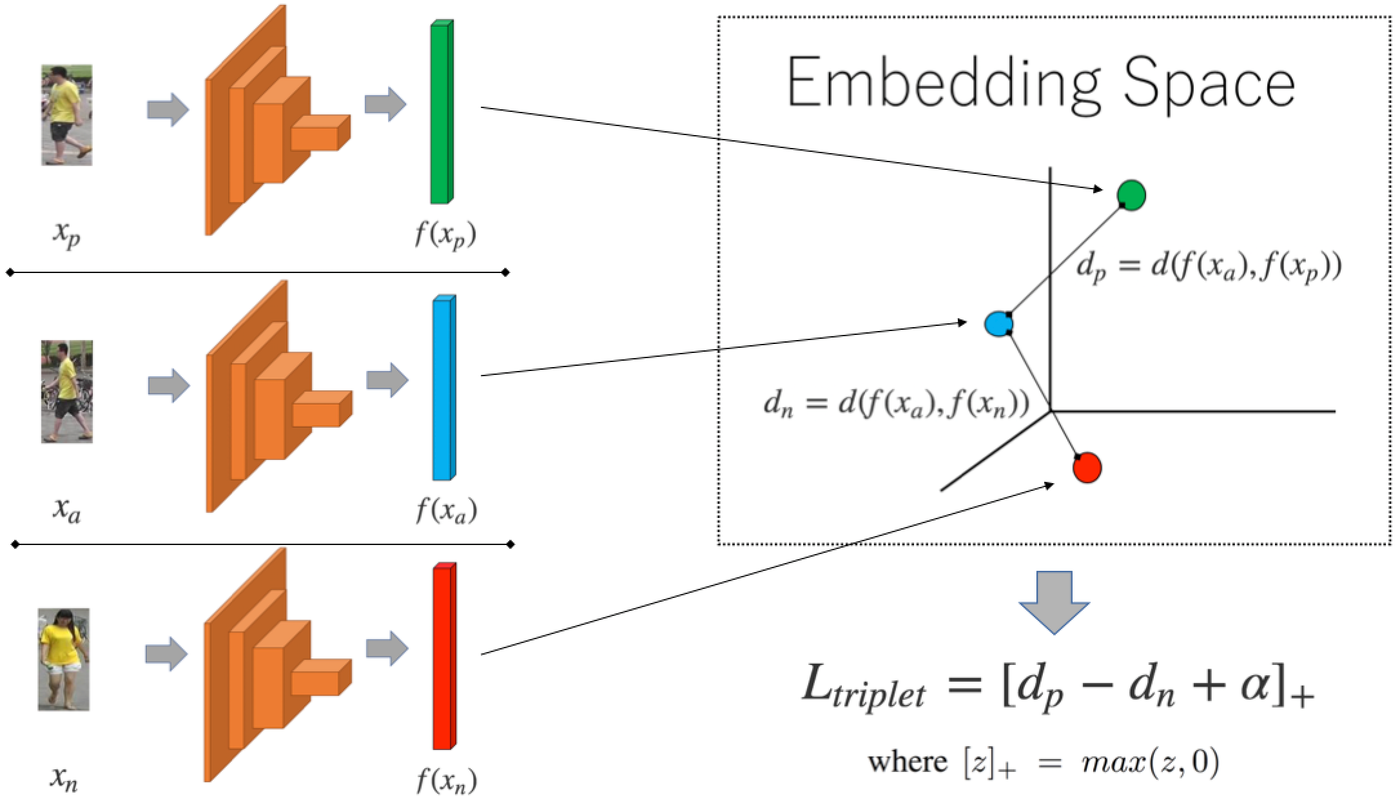
\includegraphics[width=\linewidth]{01.png}
    \end{minipage}
    \captionof{figure}{Esempio del risultato che si vuole ottenere}
\end{center}

L'architetura di una rete Triplet è composta da tre rami identici, che condividono gli stessi pesi e mappano gli elementi in codici $\Phi(I_i)$, $\Phi(I_j)$, $\Phi(I_k)$.

\begin{center}
    \begin{minipage}{0.5\linewidth}
    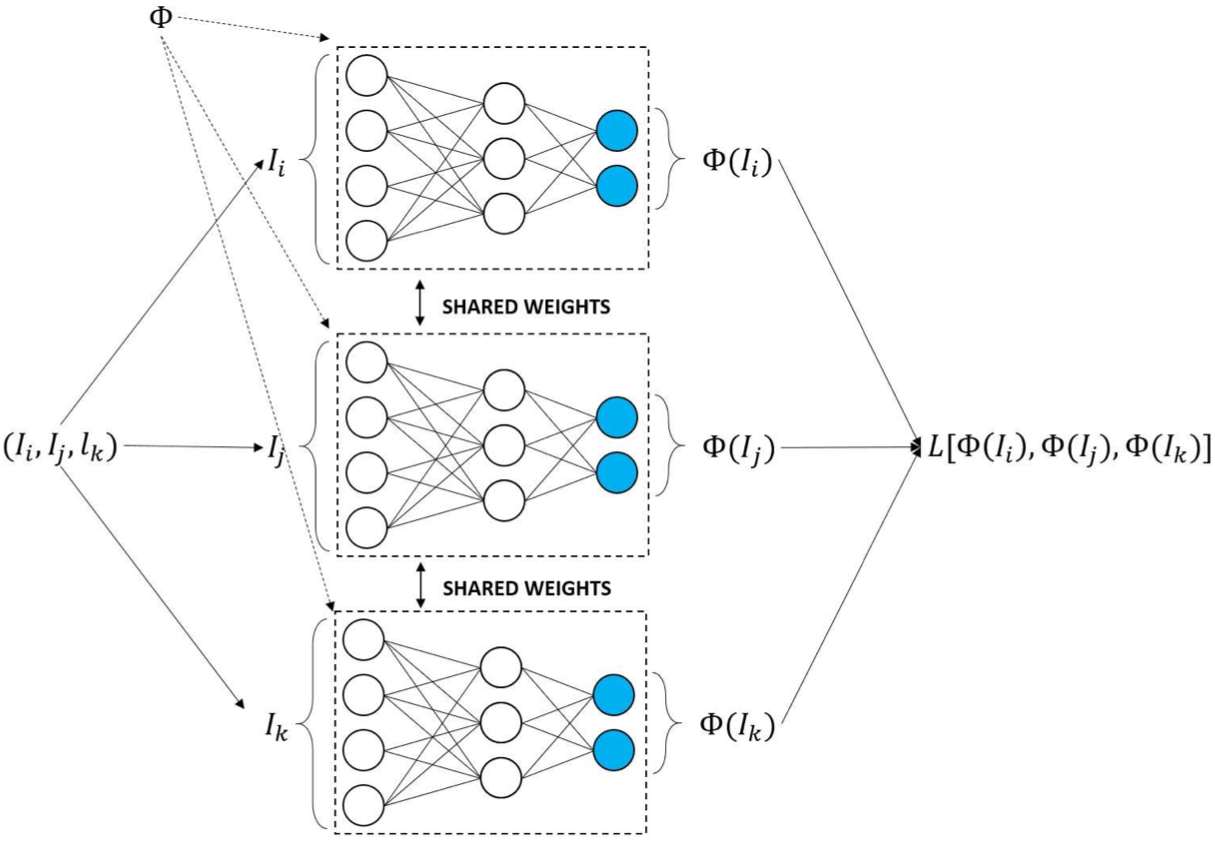
\includegraphics[width=\linewidth]{02.png}
    \end{minipage}
    \captionof{figure}{Architettura rete triplet}
\end{center}


Prende in input una tripletta di elementi $(I_i, I_j, I_k)$ che sono:

\begin{itemize}
    \item L'ancora $I_i$ 
    \item L'esempio positivo $I_j$ (che in breve ha la stessa classe di $I_i$)
    \item L'esempio negativo $I_k$, cioé un elemento diverso dalle classi di $I_i$, $I_j$
\end{itemize}

In breve, la distanza dall'ancora al positivo è minimizzata e
la distanza dall'ancora al negativo è massimizzata.
Il modello farà in modo che una coppia di campioni con le stesse etichette abbia una distanza inferiore rispetto a una copppia di campioni con etichette diverse.

\subsection{Scelta del modello}

Come feature extractor si è deciso di utilizzare una \textbf{SqueezeNet} pre-trained, eliminando il layer di classificazione.

\begin{center}
    \begin{minipage}{0.48\linewidth}
    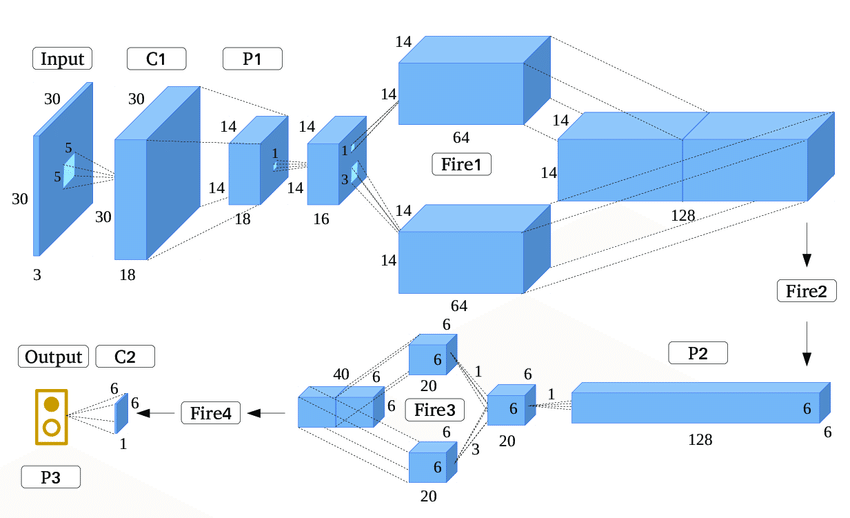
\includegraphics[width=\linewidth]{03.png}
    \end{minipage}
    \captionof{figure}{Architettura SqueezeNet}
\end{center}

Nel progetto precedente, sono stati presi in esame alcuni modelli pretrained, disponibili su
\texttt{torchvision.models}, per effettuare il task di classificazione: per tale motivo,
è stato più conveniente utilizzare \texttt{SqueezeNet}, che aveva comunque ottenuto il miglior risultato
in termini di tempo, esecuzione e validazione.

Inizialmente, nonostante la maggiore potenza computazionale rispetto allo studio precedente,
sono state effettuate delle prove utilizzando \texttt{MobileNetV2}, ma quest'ultima richiedeva
circa il doppio del tempo di \texttt{SqueezeNet}

In particolare, il completamento di un'epoca utilizzando \texttt{MobileNetV2} richiedeva 70 minuti
contro i 35/40 di \texttt{SqueezeNet v1} per immagini a colori \texttt{224x224}. Approssimando ed effettuando un training di 60 epoche \texttt{SqueezeNet v1} impiegherebbe 30 ore contro le 70 di \texttt{MobileNetV2}.

\subsection{Ottimizzazione del modello}

Sono state utilizzate funzioni, presenti su \texttt{pytorch-lighting} per trovare automaticamente i parametri da usare per il training del modello.
Nel dettaglio:

\begin{itemize}
    \item {\textbf{Batch Size Finder} 
        impiegato per evitare problemi in memoria durante il training. Viene utilizzato
        per trovare la dimensione batch più grande, che si adatta alla memoria. In questo caso il pc supportava batch di dimensioni fino a \textbf{6600} I lotti di grandi
        dimensioni spesso producono una migliore stima dei gradienti,
        ma possono anche comportare tempi di addestramento più lunghi. Dopo diverse prove è stato
        opportuno fissarla a \textbf{256}; 
    }
    \item \textbf{Learning Rate Finder} {

        Selezionare un learning rate è essenziale sia per
        prestazioni migliori, che per una convergenza più rapida. Da documentazione,
        il \textit{learning rate finder} esegue una piccola run dove il learning rate viene aumentato dopo ogni batch elaborato
        e viene registrata la loss corrispondente.
    }

\end{itemize}

\section{Dataset}

Si è presentata la necessità di riadattare il dataset in triplette: ad ogni elemento di \textbf{ancora} verrà
associato un elemento \textbf{positivo} ed uno \textbf{negativo}, che sarà scelto randomicamente 
(ad esempio, se l'ancora è della classe 'vuoto', l'elemento negativo sarà scelto randomicamente tra 'pieno' o 'mezzo')
Per questo, sono state implementate delle funzioni ad-hoc il cui utilizzo è documentato su \texttt{dataset.ipynb}. 

\begin{center}
    \begin{minipage}{0.6\linewidth}
    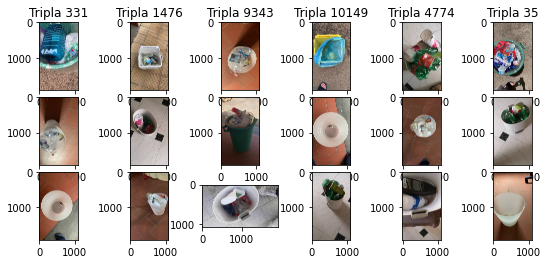
\includegraphics[width=\linewidth]{triplet_dataset.png}
    \end{minipage}
    \captionof{figure}{Dataset organizzato in triplette}
\end{center}

Effettuando vari test, è stato trovato più efficiente salvare il dataset generato in
\texttt{.csv}, evitando memorizzare le triplette in memoria. Si nota che, per incrementare
la \textbf{generalizzazione}, sarebbe utile avere a disposizione diversi
\texttt{.csv} del dataset adattato ed alternare le varie versioni del dataset dopo un certo numero di epoche, 
in quanto, la funzione è stata implementata in modo tale che le triplette generate siano diverse ad ogni esecuzione del codice. Nel nostro caso, viene utilizzata
una versione per le prime 30 epoche e successivamente viene cambiato ogni 15.

\pagebreak
\section{Scelta della loss}

Per il training della rete siamese sono state prese in esame due loss differenti (disponibili su \texttt{torch.nn})

\subsection{Triplet margin loss}
Dati in input i tensori $x_1$, $x_2$, $x_3$ ed un $margin$ con un valore $> 0$, ed è
utilizzata per misurare una similitudine tra i samples.
Una tripletta è composta da $a$ (ancora), $p$ (positivo) ed $n$ (negativo). 
\begin{center}
    \ \
    $L(a,p,n) = \max{ \{ d(a_i, p_i) - d(a_i, n_i) + margin, 0 \} }$, dove \ \
    \\
    $d(x_i, y_i) = \|| x_i - y_i ||\ _p$
    \ \
\end{center}

\subsection{Triplet margin with distance loss}
Dati in input i tensori $a$ (ancora), $p$ (positivo) ed $n$ (negativo) ed una funzione a valori
reali non negativa chiamata \textit{funzione di distanza} $d$ usata per calcolare la relazione tra
l'ancora e l'esempio positivo (distanza positiva) e l'ancora e l'esempio negativo (distanza negativa). La loss non ridotta può essere descritta dalla seguente formula:

\begin{center}
    $l(a,p,n) = L = { \{ l_1, \ldots, l_N \}}^T, l_i = \max{\{ d(a_i, p_i) - d(a_i, n_i) + margin, 0 \}} $
\end{center}

dove:

\begin{enumerate}
    \item $N$ è la dimensione del batch;
    \item {$d$ è una funzione non negativa a valori reali, che quantifica la vicinanza di due tensori riferito
    alla funzione di distanza;}
    \item {$margin$ 
        è un margine non negativo, che rappresenta la differenza minima
        tra le distanze positive e negative che è richiesto dalla loss che sia 0;
    }
    \item Il tensore di input ha $N$ elementi ognuno del quale può essere di qualsiasi forma, che la funzione di distanza può gestire.

    \item {
        Di default la funzione di distanza utilizzata è la Paiwrise Distance Funtion,
        che calcola la distanza tra i vettori $v_1$ e $v_2$ usando la p-norm:
    }
    \subitem {
        \begin{center}
            $ \| x \| _p = ( \sum^n_{i=1} |x_i|^p )^{\frac{1}{p}} $
        \end{center}
    }

\end{enumerate}


\pagebreak
\section{Training}

Durante le prime fasi di training sono state effettuate delle prove con e senza data augmentation. Inizialmente, la data augmentation applicata
era quella del progetto precedentemente citato, senza fornire miglioramenti.

Nel grafico, a 0 corrisponde vuoto, 1 metà, 2 pieno.

\begin{center}
    \begin{minipage}{0.3\linewidth}
    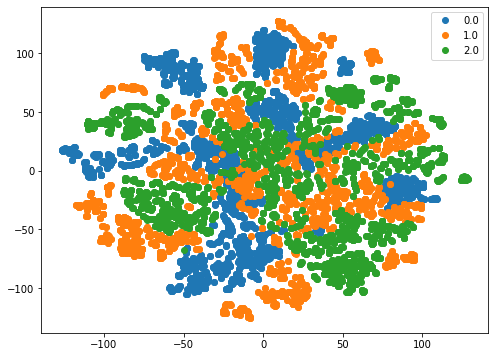
\includegraphics[width=\linewidth]{04.png}
    \end{minipage}
    \begin{minipage}{0.3\linewidth}
    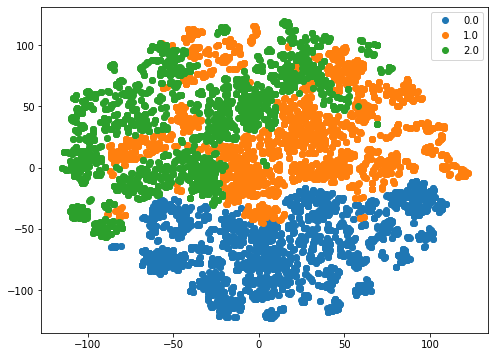
\includegraphics[width=\linewidth]{05.png}
    \end{minipage}
    \begin{minipage}{0.3\linewidth}
    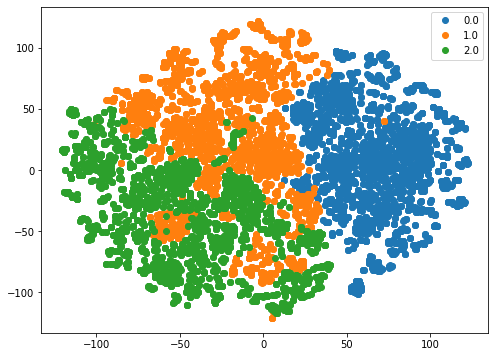
\includegraphics[width=\linewidth]{06.png}
    \end{minipage}
    \captionof{figure}{Embedding di elementi randomici sul dataset \textbf{senza data augmentation}, rispettivamente dopo: 0, 10, 30 epoche di training, utilizzando Triplet Margin Loss}
\end{center}


\begin{center}
    \begin{minipage}{0.3\linewidth}
    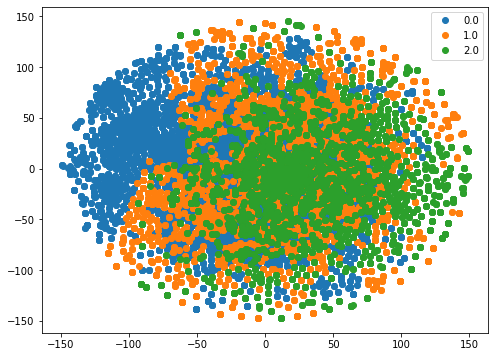
\includegraphics[width=\linewidth]{07.png}
    \end{minipage}
    \begin{minipage}{0.3\linewidth}
    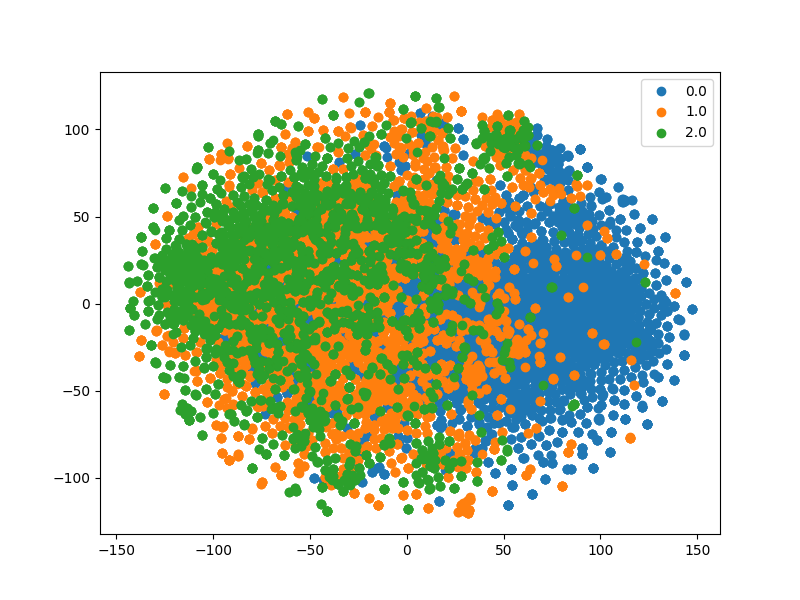
\includegraphics[width=\linewidth]{08.png}
    \end{minipage}
    \begin{minipage}{0.3\linewidth}
    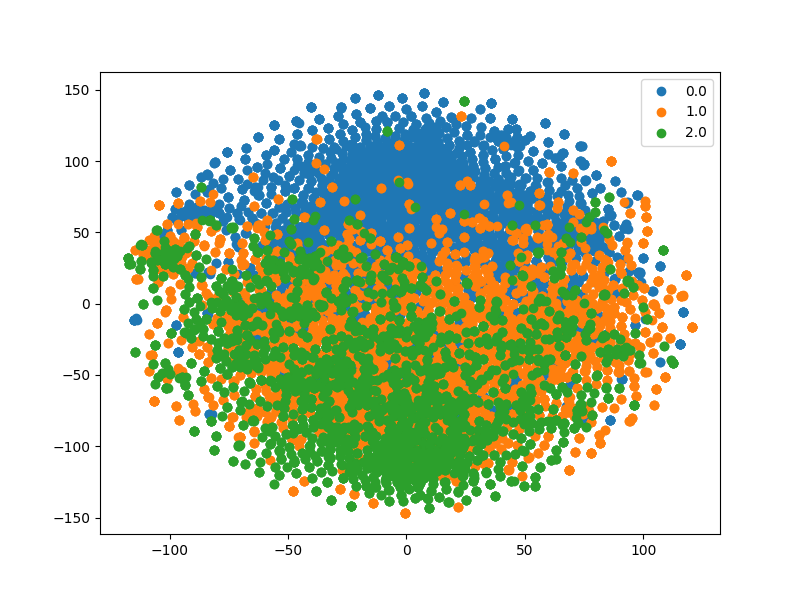
\includegraphics[width=\linewidth]{09.png}
    \end{minipage}
    \captionof{figure}{Embedding di elementi randomici sul dataset \textbf{con data augmentation forte}, rispettivamente dopo: 0, 30, 60 epoche di training, utilizzando Triplet Margin Loss}
\end{center}

Dopo numerose prove, è stato opportuno applicare \texttt{RandomCrop()} e \texttt{RandomPerspective} al dataset di training e \texttt{CenterCrop} al dataset di test

\pagebreak

Gli errori classificazione ottenuti dalle loss due loss sono riassunti nella seguente tabella:

\begin{center}
    \begin{tabular}{ | l | l | l | p{5cm} |}
    \hline
    Epoch & Triplet Margin Loss & Triplet Margin With Distance Loss \\ \hline
    0 & 0.677 & 0.739 \\ \hline
    15 & 0.936 & 0.792: \\ \hline
    30 & 0.900 & 0.894  \\
    \hline
    \end{tabular}
\end{center}

\begin{center}
    \begin{minipage}{0.3\linewidth}
    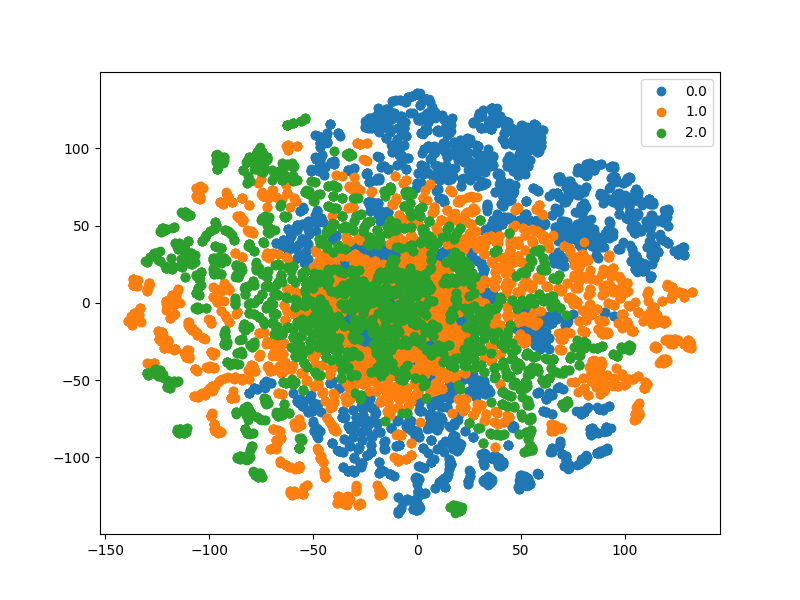
\includegraphics[width=\linewidth]{TML-TSNE-0.png}
    \end{minipage}
    \begin{minipage}{0.3\linewidth}
    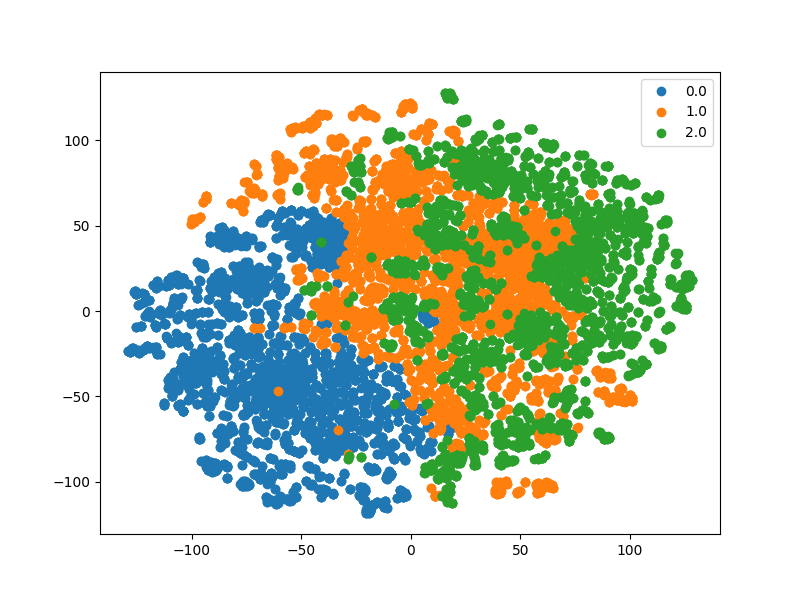
\includegraphics[width=\linewidth]{TML-TSNE-15.png}
    \end{minipage}
    \begin{minipage}{0.3\linewidth}
    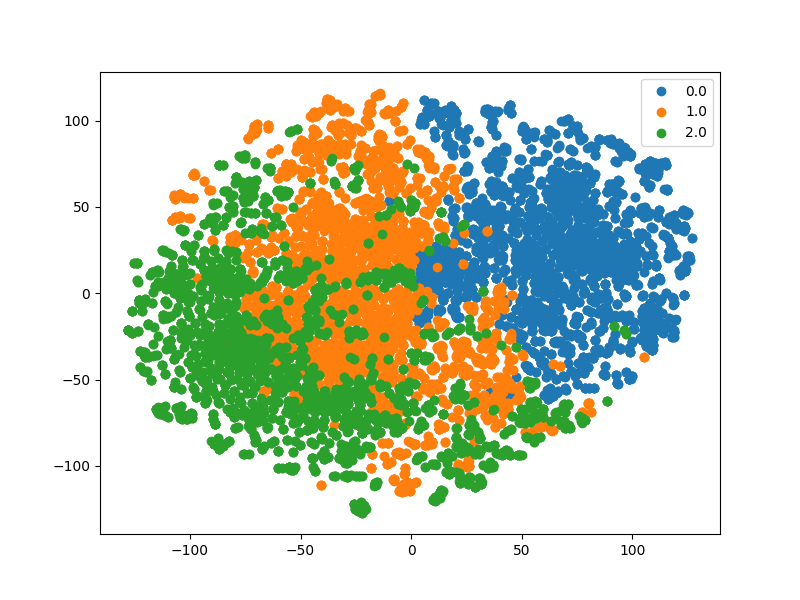
\includegraphics[width=\linewidth]{TML-TSNE-30.png}
    \end{minipage}
    \captionof{figure}{Embedding di elementi randomici sul dataset utilizzando il modello con \textbf{Triplet Margin Loss}, rispettivamente dopo: 0, 15, 30 epoche di training}    
\end{center}

\begin{center}
    \begin{minipage}{0.3\linewidth}
    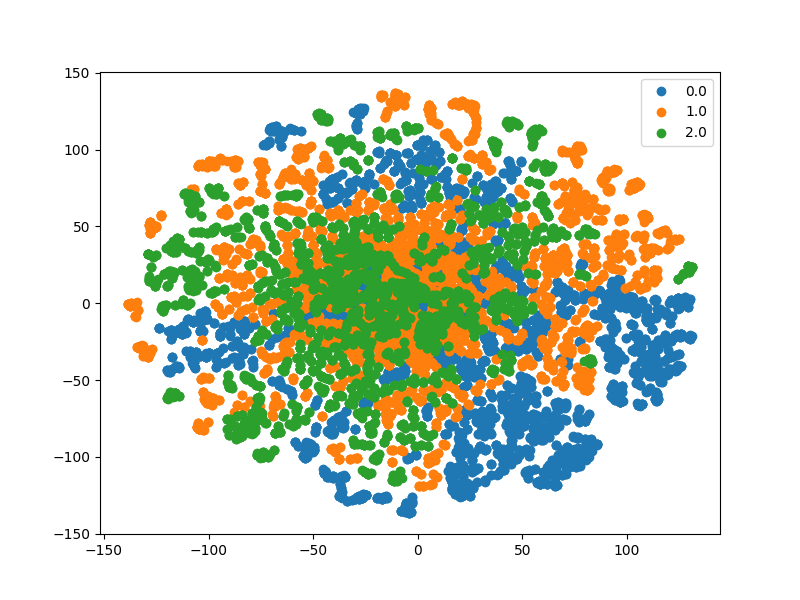
\includegraphics[width=\linewidth]{TMWDL-TSNE-0.png}
    \end{minipage}
    \begin{minipage}{0.3\linewidth}
    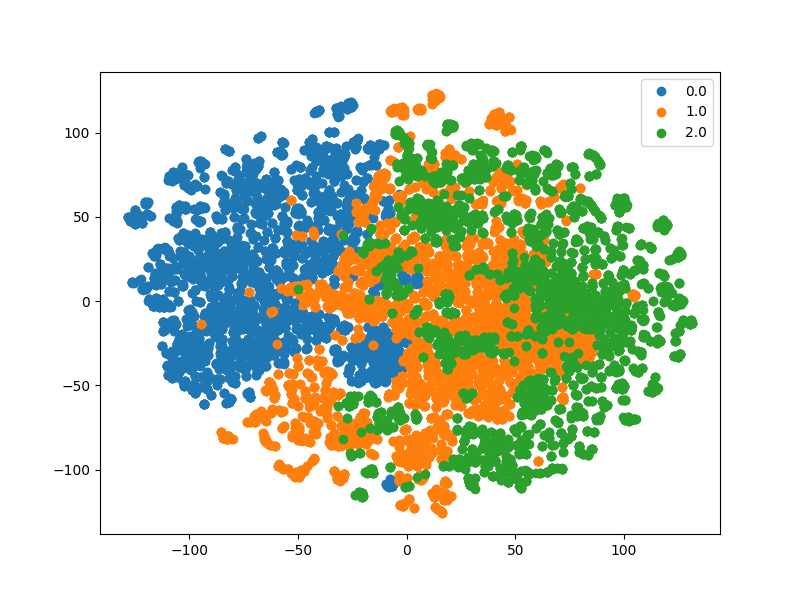
\includegraphics[width=\linewidth]{TMWDL-TSNE-15.png}
    \end{minipage}
    \begin{minipage}{0.3\linewidth}
    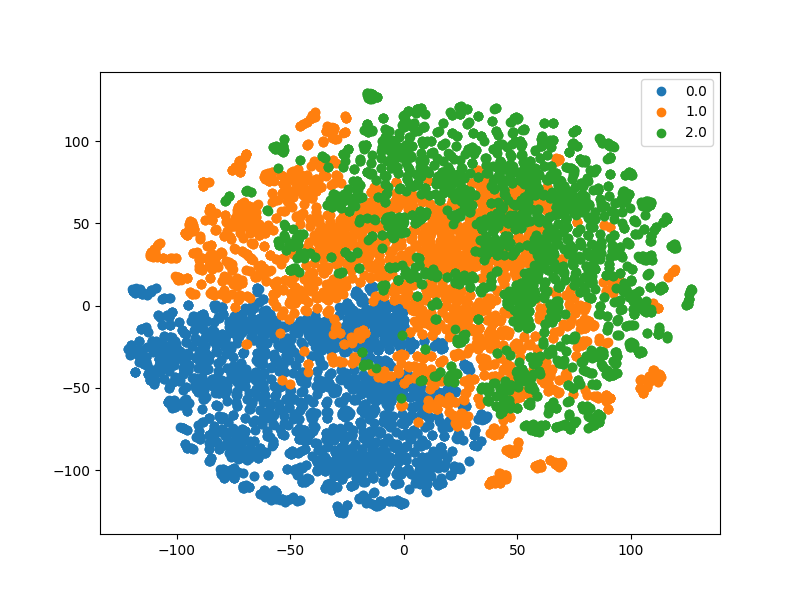
\includegraphics[width=\linewidth]{TMWDL-TSNE-30.png}
    \end{minipage}
    \captionof{figure}{Embedding di elementi randomici sul dataset utilizzando il modello con \textbf{Triplet Margin with Distance Loss}, rispettivamente dopo: 0, 15, 30 epoche di training}    
\end{center}

\begin{center}
    \begin{minipage}{0.3\linewidth}
    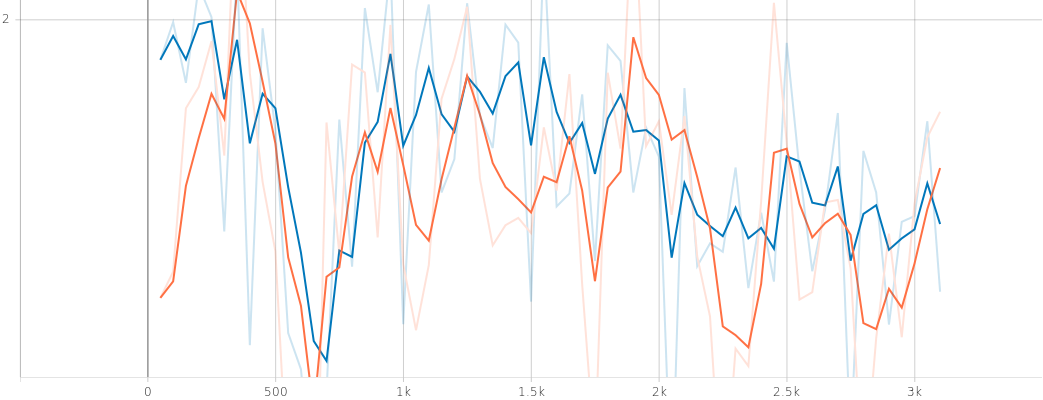
\includegraphics[width=\linewidth]{train_loss.png}
    \end{minipage}
    \begin{minipage}{0.3\linewidth}
    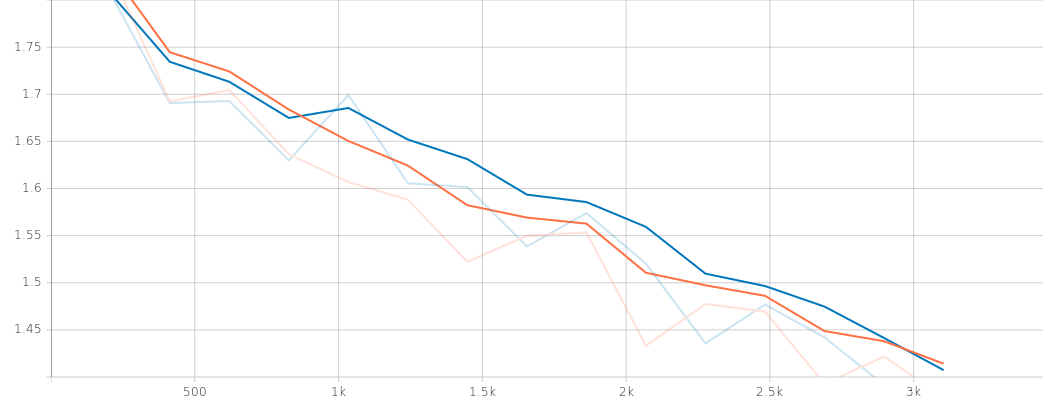
\includegraphics[width=\linewidth]{valid_loss.png}
    \end{minipage}
    \captionof{figure}{Grafici di convergenza di training (sx) e validation (dx) del modello utilizzando Triplet Margin Loss (arancione) e Triplet Margin with Distance Loss (blu)}
\end{center}


\pagebreak
\section{Conclusione}

Nonostante nell'immediato la triplet margin with distance loss ottenga, a parità di epoca, un punteggio migliore rispetto (di pochissimo)
alla triplet margin loss,
si decide comunque di procedere continunando il training con la triplet margin loss in quanto, visualizzando il grafico,il valore della loss
è diminuito molto di più rispetto all'altra.
Per aumentare la generalizzazione, inoltre, ogni 15 epoche il dataset utilizzato per effettuare il training verrà cambiato. 

\begin{center}
    visualizzazione dei grafici dei tnse completi
\end{center}


\begin{center}
    \begin{minipage}{0.3\linewidth}
    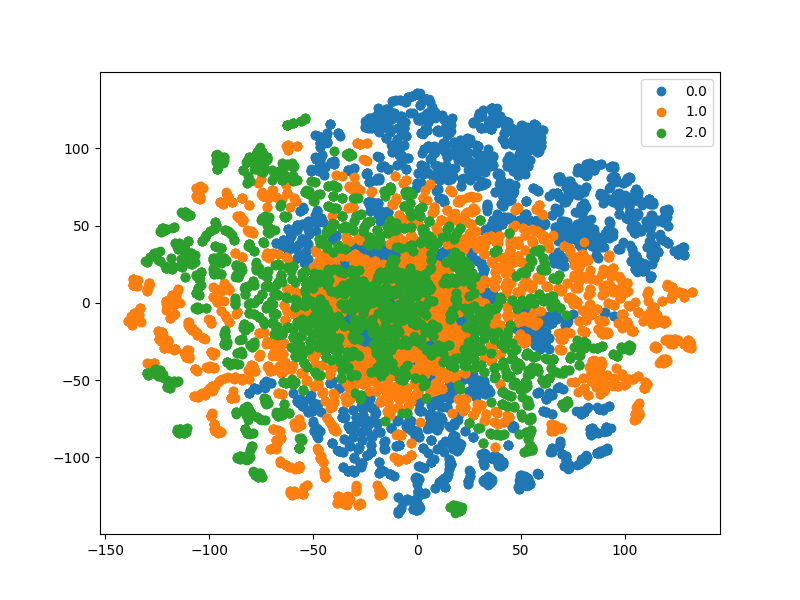
\includegraphics[width=\linewidth]{TML-TSNE-0.png}
    \end{minipage}
    \begin{minipage}{0.3\linewidth}
    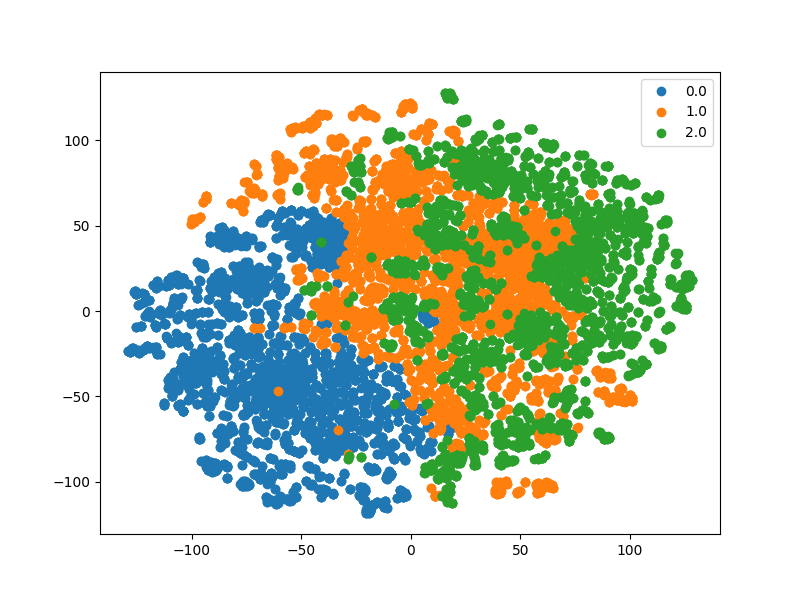
\includegraphics[width=\linewidth]{TML-TSNE-15.png}
    \end{minipage}
    \begin{minipage}{0.3\linewidth}
    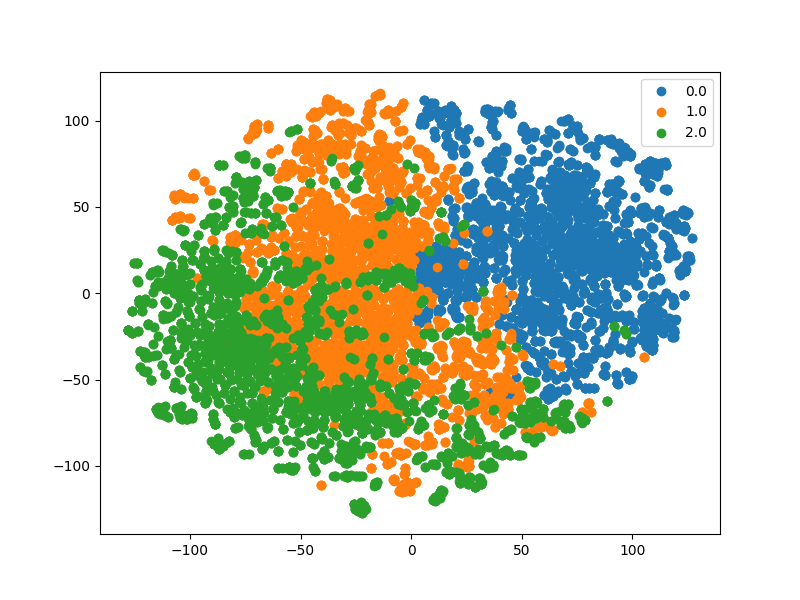
\includegraphics[width=\linewidth]{TML-TSNE-30.png}
    \end{minipage}
    \begin{minipage}{0.3\linewidth}
    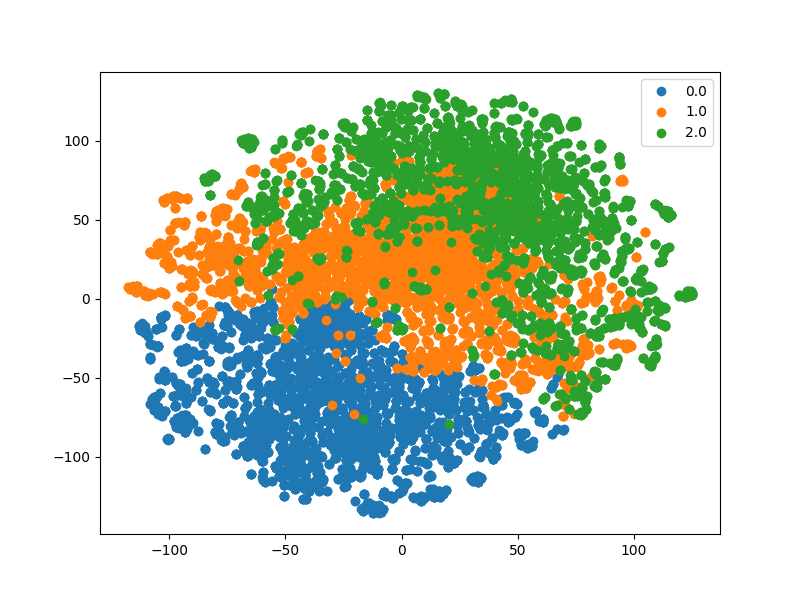
\includegraphics[width=\linewidth]{TML-TSNE-45.png}
    \end{minipage}
    \begin{minipage}{0.3\linewidth}
    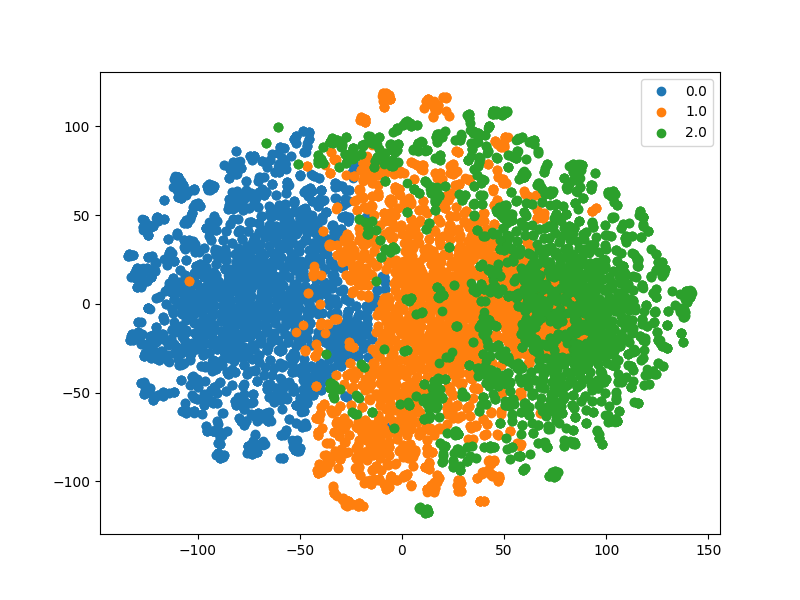
\includegraphics[width=\linewidth]{TML-TSNE-60.png}
    \end{minipage}
    \captionof{figure}{Embedding di elementi randomi utilizzando Triplet Margin loss rispettivamente dopo: 0, 15, 30, 40, 60 epoche di training}
\end{center}

\begin{center}
    grafo di convergenza finale
\end{center}

\begin{center}
    \begin{minipage}{0.48\linewidth}
    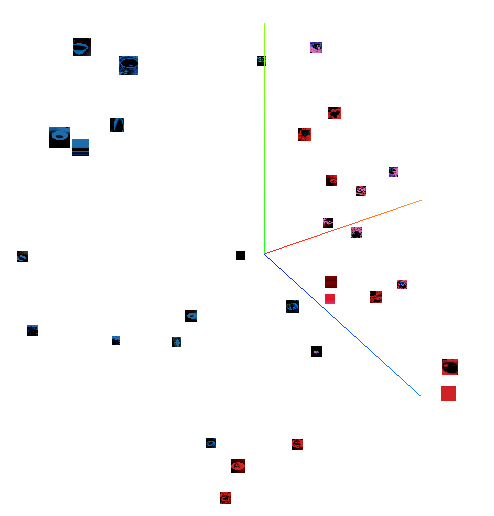
\includegraphics[width=\linewidth]{tensorboard_2.png}
    \end{minipage}
    \captionof{figure}{Visualizzazione embedding 3D}
\end{center}

Errore di validazione / classificazione finale


\pagebreak

\begin{thebibliography}{4}

\bibitem{1} \href{https://pytorch.org/vision/stable/models.html}{Models and Pre-trained Weights}
\bibitem{2} \href{
    https://pytorch.org/docs/stable/generated/torch.nn.TripletMarginLoss.html
}{Triplet Margin Loss}
\bibitem{2} \href{
    https://pytorch.org/docs/stable/generated/torch.nn.TripletMarginWithDistanceLoss.html#torch.nn.TripletMarginWithDistanceLoss
}{Triplet Margin With Distance Loss}
\bibitem{4} \href{
    https://pytorch.org/docs/stable/generated/torch.nn.PairwiseDistance.html
}{PairwiseDistance}

% https://openaccess.thecvf.com/content_CVPR_2020/papers/Ko_Embedding_Expansion_Augmentation_in_Embedding_Space_for_Deep_Metric_Learning_CVPR_2020_paper.pdf


\end{thebibliography}


\pagebreak
%--/Paper--

\end{document}
